\documentclass[11pt]{report}

\usepackage[latin1]{inputenc} % un package
\usepackage[T1]{fontenc}      % un second package
\usepackage[francais]{babel}  % un troisi�me package
\usepackage{lmodern}
\usepackage{graphicx}

%%%% debut macro pour enlever le nom chapitre %%%%
\makeatletter
    \def\@makechapterhead#1{%
        \vspace*{50\p@}%
        {\parindent \z@ \raggedright \normalfont
            \interlinepenalty\@M
            \ifnum \c@secnumdepth >\m@ne
            \Huge\bfseries \thechapter\quad
            \fi
            \Huge \bfseries #1\par\nobreak
            \vskip 40\p@
        }}

    \def\@makeschapterhead#1{%
        \vspace*{50\p@}%
        {\parindent \z@ \raggedright
            \normalfont
            \interlinepenalty\@M
            \Huge \bfseries  #1\par\nobreak
            \vskip 40\p@
        }
    }
\makeatother
%%%% fin macro %%%%


\begin{document}

\begin{titlepage}
\centering

\setcounter{page}{0} % enlever num�ro de page

 
\textbf{Yacine Maghezzi}\\ 
Licence 3 Informatique\\
D�partement de Math�matique et Informatique\\

\vspace{4cm}

\small Rapport de Stage \\
\LARGE Application mobile Yuukou et gUSE\\
\vspace{1cm}

\includegraphics[scale=0.25]{img/wmin.jpg} 

\vspace{4cm}


\noindent 
\center{Maitre de stage : M. Thierry Delaitre\\
Tuteur de stage : M. Jean-Michel Hufflen\\ 
}
\vspace{1cm}
\textbf{Lieu de stage :} University Of Westminster\\
\textbf{Dur�e/Date :}12 mars - 3 Juin\\


\end{titlepage}
\clearpage

\tableofcontents
\chapter{Introduction}

A L'Universit� de Besan�on, les �tudiants de Licence 3 Informatique
sont amen�s � r�aliser un stage en entreprise d?une dur�e minimum
de 3 mois. Il est possible aux �tudiants de r�aliser ce stage dans un pays
�tranger.
Cela a �t� l'occasion de pouvoir am�liorer grandement mon anglais, ainsi que ma connaissance de la culture du pays.
J'ai eu la chance de obtenir mon stage par l'interm�diaire
de M. Jean-Michel Hufflen, Ma�tre de Conf�rences � l?Universit� de Besan�on, un stage au sein de l?Universit� de Westminster � Londres o� j?ai �t� accueilli dans l?�quipe du Centre for Parallel Computing par M. Thierry Delaitre, directeur des infrastructures � l?universit�.\\

Durant ce stage, j'ai �t� amen� � travailler sur deux sujets de stage. Le
premier avait pour sujet la r�alisation d'une application Web destin�e au plateforme mobiles. Il
consistait a rendre les ressources informatiques, ainsi qu'un certain nombre d'information au 20000 usagers quotidient du L'universit�e de Westminster.
Le deuxi�me sujet m?a �t� attribu� afin de me permettre de r�utiliser
les connaissances acquises durant le premier. Il consistait � d�velopper une
solution de gestion de machines virtuelles servant de support de cours aux
enseignants de l?Universit� de Westminster.

Le pr�sent rapport explique le travail que j?ai r�alis� durant mon stage. Il
est compos� de 5 parties expliquant dans un premier temps le cadre de mon
stage dans l?universit� et les sujets qui m?ont �t� propos�s. Je poursuis ensuite
en parlant du travail de documentation que j?ai r�alis� afin de comprendre
les outils que j?allais devoir prendre en main. Je continue en pr�sentant en
deux parties le travail r�alis� sur chacun des deux sujets. Je termine par deux
derni�res parties pour tirer le bilan de ce stage avant de conclure ce rapport.
\clearpage
\chapter{Remerciements}

Je tiens � remercier certaines personnes sans qui ce stage n?aurait pas pu
avoir lieu et se d�rouler dans de bonnes conditions.
\vspace{1cm}

\begin{itemize}

\item Je voudrais remercier M. Thierry Delaitre mon ma�tre de stage pour
son accueil au sein de l?Universit� de Westminster, pour l?encadrement
de mon stage et pour ses conseils pour la r�alisation de ce dernier.
\vspace{1cm}

\item Je remercie �galement. Jean-Michel Hufflen, Maitre de Conf�rences
� l'Universit� de Besan�on pour m?avoir aid� � trouver ce stage et pour
m?avoir aid� � corriger le pr�sent rapport.

\vspace{1cm}
\item Je tiens a remercier mon coll�gue Benoit Meihlac pour son aide, car sans lui la compr�hension du web-service qu'il a cr�e aurait �t� difficile.

\vspace{1cm}
\item Je remercie �galement mon camarade, Damien Hostache pour sa compagnie amicale
durant le stage.
\end{itemize}
\clearpage
\chapter{London}

\section{University of Westminster}

\subsection{Pr�sentation}

L'Universit� de Westminster a �t� cr��e en 1838 par M. George Cayley
et avait pour nom Royal Polytechnic Institution. Cette �cole fut le premier lieu d?enseignement technique en Grande-Bretagne.

\begin{figure}[h!]
  \centering
      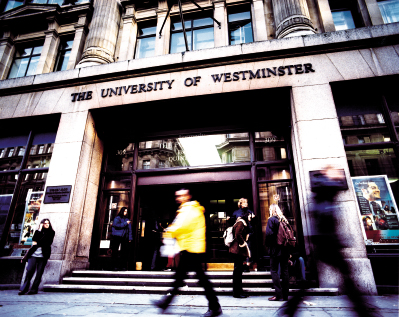
\includegraphics[width=0.9\textwidth]{img/wmin2.jpg}
  \caption{Le campus principal}
\end{figure}
TODO completer pr�sentation

\subsection{Campus et �coles}
L'Universit� de Westminster est actuellement compos� de 6 sites r�partis
dans Londres et ses environs.
\begin{itemize}

\item Le site Cavendish qui se trouve au 101-115 New Cavendish Street
proche de la tour de la British Telecom. Il contient deux �coles :
\begin{itemize}
\item Sciences de la vie
\item Electronique et informatique
\end{itemize}

C'est dans ce site que mon stage s'est d�roul� au sein de l'�cole �lectronique
et Informatique School of electronics and computer science. La figure
suivante pr�sente le b�timent vu de devant.

\begin{figure}[h!]
  \centering
      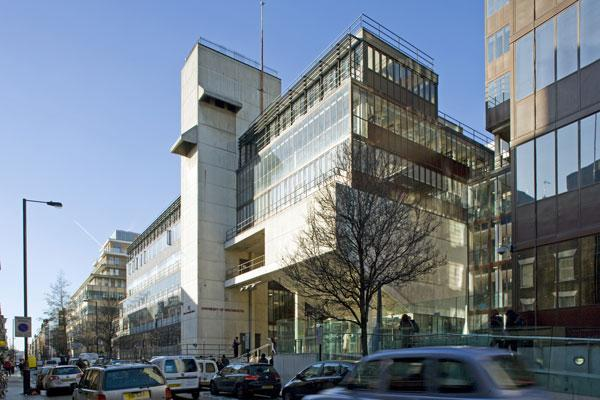
\includegraphics[width=0.9\textwidth]{img/wmin1.jpg}
  \caption{Le campus de New Cavendish Street}
\end{figure}

\item Le site de Great Portland Street se trouve au 70-74 Great Portland
street, il contient le d�partement du centre informatique pour personnes
handicap�es.
\item Le site de Harrow se trouve � Watford road. Il contient deux �coles :

\begin{itemize}
\item une partie de l'�cole d'�lectronique et informatique
\item l'�cole des m�dias, de l'art et du design
\end{itemize}

\item Le site de Little Titchfield Street se trouve au 4-12 Little Titchfield
street, il contient l'�cole de droit.
\item Le site de Marylebone se trouve au 35 Marylebone road. Il contient
l'�cole d'architecture et de construction environnementale.
\item Le site de Regent Street qui se trouve au 309 Regent street est le plus
ancien site de l'universit�. Il comprend l'�cole des sciences sociales, des
sciences humaines et des langues.
\end{itemize}


\subsection{School of Electronics and Computer Science}
Cette �cole est en cohabitation avec l'�cole de sciences de la vie au
sein du site de Cavendish. On peut voir que cette �cole est constitu�e de
d�partements et de 4 groupes de recherches dont voici les �nonces :
\begin{itemize}
\item Department of Business Information Systems
\item Department of Computer Science and Software Engineering
\item Department of Electronic, Network and Computer Engineering
\item Electronic and Communication Engineering
\item Operational Research and Intelligent Systems
\item Parallel and Distributed Computing
\item Semantic Computing and Systems Engineering
\end{itemize}
Cette �cole est tr�s r�put�e pour les programmes d'�changes internationaux.
J?ai pu y d�couvrir nombre d'�tudiants �trangers qui viennent �tudier
dans ce site.
L'�cole propose beaucoup de domaines d'enseignement dans le parcours
informatique. Il est ainsi possible de suivre des cours de gestion de syst�mes
d'information, de programmation parall�le et distribu�e, de programmation
d'intelligence artificielle en passant �galement par le d�veloppement de jeux
vid�os et d'autres formations.


\subsection{Informations et chiffres}

Avec un peu plus de 24000 �tudiants, l'universit� de Westminster fait partie des universit� les plus prestigieuses du Royaume Uni.
L'universit� compte quelques dipl�m�s de prestiges, avec des grands nom tel que Cherie Blair, senior barrister, femme de Tony Blair,
TO DO, Completer cette partie
 




\clearpage
\chapter{Pr�sentation du sujet}
\section{Le projet Yuukou}
\subsection{Pr�sentation}

Yuukou, du japonais qui d�signe la validit� (e), la disponibilit�, l'efficacit�, est un syst�me qui recueille des informations d'authentification � partir de serveurs LDAP afin de comprendre et de construire l'infrastructure des ressources et permet de facilit� son utilisation. Yuukou est �t� cr�� pour faciliter l'utilisation des laboratoires informatiques � l'Universit� de Westminster.





\clearpage

\end{document}

